%==============================================================================
% PAPER 6, CHAPTER 1: Quantum Computing Applications
%==============================================================================

\chapter{Quantum Computing Applications}
\label{ch:p6:quantum_computing}

%------------------------------------------------------------------------------
\section{Introduction: The Polynomial-Time Promise}
%------------------------------------------------------------------------------

\openingquote{%
``The question is, what kind of physical laws permit the existence of algorithms that compute things exponentially faster than classical algorithms?''%
}{Peter Shor, 1994}

\marginnote{historical-context}{%
Shor's 1994 discovery that quantum computers can factor integers in polynomial time sparked the quantum computing revolution, threatening RSA cryptography.%
}

In 1994, Peter Shor announced a result that sent shockwaves through cryptography and computer science: a quantum algorithm for factoring integers in time polynomial in the number of digits\cite{Shor1994}. Classical factoring algorithms, such as the general number field sieve, require sub-exponential time $\exp(O(n^{1/3}\log^{2/3} n))$ for $n$-bit integers. Shor's algorithm achieves $O(n^3)$ time using quantum Fourier transforms and period-finding---an exponential speedup.\marginnote{physical-intuition}{%
Quantum parallelism allows simultaneous evaluation of function values across exponentially many inputs encoded in superposition states.%
}

The implications were immediate: RSA encryption, foundation of internet security, relies on the computational hardness of factoring large semiprimes (products of two large primes). A sufficiently powerful quantum computer---estimated at $\sim10^7$ physical qubits after error correction---could break 2048-bit RSA in hours.\marginnote{computational-complexity}{%
Factoring is in BQP (bounded-error quantum polynomial time) but believed not in P (deterministic polynomial time), creating separation between quantum and classical complexity classes.%
}

Yet practical quantum computing faces a formidable obstacle: \textit{decoherence}. Quantum states are fragile, collapsing under environmental interaction on microsecond timescales for superconducting qubits, seconds for trapped ions. Current state-of-the-art coherence times:\marginnote{experimental-status}{%
As of 2025, coherence times: superconducting $T_2 \sim 200~\mu$s, trapped ions $T_2 \sim 10$ s, NV centers $T_2 \sim 1$ ms (room temp).%
}

\begin{equation}
  T_2^{\text{SC}} \sim 100{-}200~\mu\text{s}, \quad T_2^{\text{ion}} \sim 1{-}10~\text{s}, \quad T_2^{\text{NV}} \sim 10^{-3}{-}10^{-1}~\text{s}
  \label{eq:p6:coherence_times}
\end{equation}

Running Shor's algorithm for 2048-bit factorization requires $\sim10^7$ gate operations over milliseconds to seconds, demanding aggressive error correction. Surface codes---the leading approach---impose $\sim10^3:1$ physical-to-logical qubit overhead, rendering near-term factorization infeasible.\marginnote{engineering-challenge}{%
IBM's 433-qubit Osprey processor (2022) provides $<1$ logical qubit after error correction, illustrating the resource gap.%
}

This chapter explores how advanced theoretical physics---topological quantum states, exceptional algebraic structures, and non-integer dimensional quantum walks---offers pathways to enhanced quantum information processing. We ground speculation in experimental feasibility, quantify performance improvements, and outline realistic technology timelines.

%------------------------------------------------------------------------------
\section{Topological Quantum Computing}
%------------------------------------------------------------------------------

\subsection{Non-Abelian Anyons and Braiding Operations}

Topological quantum computing encodes information in global properties of quantum states, providing inherent protection against local perturbations\cite{Kitaev2003}. The key insight: quantum information stored in \textit{anyonic} quasiparticles emerging in two-dimensional systems obeys exotic exchange statistics.\marginnote{theoretical-foundation}{%
In 2D, particle exchange can be continuously deformed (braided) rather than just permuted, leading to non-Abelian statistics.%
}

For $N$ indistinguishable particles in 3D, wavefunction acquires phase $\pm1$ under exchange (bosons/fermions). In 2D, particle worldlines can \textit{braid} around each other, defining continuous group of exchanges. Wavefunctions transform under unitary representations:\marginnote{mathematical-structure}{%
Braid group $B_N$ on $N$ strands has generators $\sigma_i$ (exchange $i \leftrightarrow i+1$) satisfying $\sigma_i \sigma_j = \sigma_j \sigma_i$ for $|i-j| \geq 2$ and $\sigma_i \sigma_{i+1} \sigma_i = \sigma_{i+1} \sigma_i \sigma_{i+1}$.%
}

\begin{equation}
  |\psi\rangle \to U(\sigma_i) |\psi\rangle, \quad U(\sigma_i) \in \text{U}(d)
  \label{eq:p6:anyon_braiding}
\end{equation}

where $d$ is the anyon type's quantum dimension. For non-Abelian anyons ($d > 1$), braiding operations perform unitary transformations in degenerate ground-state subspace---quantum gates protected from local errors.\marginnote{error-protection}{%
Local perturbations cannot distinguish between degenerate ground states separated by topological gap $\Delta \sim 10$ K, providing thermal protection.%
}

\subsection{E$_8$ Lattice Anyons}

The E$_8$ exceptional Lie group, with 240 roots forming an 8-dimensional lattice, provides a natural framework for topological phases\cite{Freedman2005}. Dimensional reduction from 8D to (2+1)D via compactification yields effective anyon models with fusion rules:\marginnote{dimensional-reduction}{%
Compactification on $T^5$ torus projects E$_8$ roots onto 3D subspace, producing finite-dimensional fusion categories.%
}

\begin{equation}
  a \times b = \sum_c N_{ab}^c \, c
  \label{eq:p6:fusion_rules}
\end{equation}

where $N_{ab}^c \in \mathbb{Z}_{\geq 0}$ counts fusion channels. For E$_8$ anyons, the fusion algebra generates 240 distinct particle types corresponding to root vectors. Specific reduced models include:\marginnote{physical-realization}{%
E$_8$ anyons may emerge in spin liquids or fractional quantum Hall states at exotic filling factors.%
}

\begin{itemize}
  \item \textbf{Fibonacci anyons:} Fusion rule $\tau \times \tau = 1 + \tau$ with golden ratio quantum dimension $d_\tau = (1+\sqrt{5})/2$. Universal for quantum computation\cite{Nayak2008}.

  \item \textbf{Ising anyons:} Three types $\{1, \sigma, \psi\}$ with $\sigma \times \sigma = 1 + \psi$. Requires ancilla qubits for universality.

  \item \textbf{Metaplectic anyons:} SO(3)$_3$ level theory, universal with magic state injection.
\end{itemize}

The computational advantage: braiding $N$ Fibonacci anyons generates braid group $B_N$ representations dense in SU(2) rotations, approximating arbitrary single-qubit gates to precision $\epsilon$ using $O(\log(1/\epsilon))$ braids (polynomial overhead).\marginnote{algorithm-complexity}{%
Compare to Solovay-Kitaev decomposition requiring $O(\log^{3.97}(1/\epsilon))$ gates for arbitrary rotations from discrete gate set.%
}

%------------------------------------------------------------------------------
\section{Surface Codes and Stabilizer Formalism}
%------------------------------------------------------------------------------

\subsection{Toric Code Construction}

Surface codes provide fault-tolerant quantum memory by encoding logical qubits into 2D lattices of physical qubits\cite{Dennis2002}. The \textit{toric code}---simplest surface code---places qubits on edges of square lattice on torus topology.\marginnote{topological-encoding}{%
Logical states correspond to homologically distinct loops wrapping torus, protected by topological gap.%
}

For $L \times L$ lattice (total $2L^2$ qubits), define stabilizer generators:\marginnote{stabilizer-operators}{%
Stabilizers commute with all logical operators but detect errors by anti-commuting with physical Pauli errors.%
}

\begin{align}
  A_v &= \prod_{e \in \text{star}(v)} X_e, \quad \text{(vertex operators)} \label{eq:p6:vertex_stabilizer}\\
  B_p &= \prod_{e \in \partial p} Z_e, \quad \text{(plaquette operators)} \label{eq:p6:plaquette_stabilizer}
\end{align}

where star$(v)$ denotes edges touching vertex $v$, and $\partial p$ is boundary of plaquette $p$. The $2L^2 - 2$ independent stabilizers constrain physical Hilbert space $\mathcal{H}_{\text{phys}} = (\mathbb{C}^2)^{\otimes 2L^2}$ to codespace:\marginnote{code-dimension}{%
Logical Hilbert space dimension: $\dim \mathcal{H}_{\text{log}} = 2^{2L^2} / 2^{2L^2 - 2} = 4$, encoding 2 logical qubits.%
}

\begin{equation}
  \mathcal{H}_{\text{log}} = \{|\psi\rangle \in \mathcal{H}_{\text{phys}} : A_v |\psi\rangle = |\psi\rangle, \, B_p |\psi\rangle = |\psi\rangle \, \forall v,p\}
  \label{eq:p6:logical_subspace}
\end{equation}

Logical operators are non-contractible loops:\marginnote{logical-operations}{%
Logical $\bar{X}$ winds around torus horizontally, $\bar{Z}$ vertically, anti-commuting as required for qubit algebra.%
}

\begin{equation}
  \bar{X} = \prod_{e \in \gamma_x} X_e, \quad \bar{Z} = \prod_{e \in \gamma_z} Z_e
  \label{eq:p6:logical_operators}
\end{equation}

where $\gamma_x, \gamma_z$ are homologically independent loops.

\subsection{Error Detection and Syndrome Extraction}

Errors $E$ (Pauli $X, Y, Z$ on individual qubits) anti-commute with stabilizers, flipping syndrome measurement outcomes:\marginnote{syndrome-measurement}{%
Projective measurement of $A_v, B_p$ collapses state to $\pm1$ eigenspaces without revealing logical information.%
}

\begin{equation}
  \langle A_v \rangle = \begin{cases}
    +1 & \text{no error at } v\\
    -1 & \text{error detected at } v
  \end{cases}
  \label{eq:p6:syndrome}
\end{equation}

Error syndrome is binary string $s \in \{0,1\}^{2L^2-2}$ indicating violated stabilizers. Classical decoder (e.g., minimum-weight perfect matching) infers error chain $E$ from syndrome, applies correction $E^\dagger$.\marginnote{decoding-complexity}{%
Minimum-weight perfect matching runs in $O(n^3)$ for $n$ qubits using Blossom algorithm\cite{Edmonds1965}.%
}

\textbf{Error threshold:} Surface codes tolerate physical error rate $p < p_{\text{th}} \sim 1\%$ (numerical studies). For $p < p_{\text{th}}$, logical error rate:\marginnote{threshold-theorem}{%
Threshold depends on error model: $p_{\text{th}} \sim 1.1\%$ for depolarizing noise, $\sim 2\%$ for erasure errors.%
}

\begin{equation}
  p_{\text{log}} \sim \left(\frac{p}{p_{\text{th}}}\right)^{\lceil (d+1)/2 \rceil}
  \label{eq:p6:logical_error_rate}
\end{equation}

where $d = L$ is code distance (minimum weight of logical operator). For distance-$d$ code, can correct $\lfloor (d-1)/2 \rfloor$ errors.

%------------------------------------------------------------------------------
\section{Worked Example: Distance-3 Surface Code}
%------------------------------------------------------------------------------

\subsection{Setup and Stabilizers}

Consider minimal non-trivial surface code with distance $d=3$ on planar patch (sacrificing one encoded qubit for boundary).\marginnote{planar-vs-toric}{%
Planar codes use open boundaries, simpler for physical implementation but encode fewer logical qubits per physical qubit.%
}

\textbf{Lattice:} $3 \times 3$ plaquettes require $9 + 12 = 21$ data qubits (9 vertex qubits + 12 edge qubits). Additional ancilla qubits measure stabilizers.\marginnote{qubit-count}{%
Total physical qubits: 21 data + 18 ancilla (9 vertex + 9 plaquette) = 39 for one logical qubit.%
}

\textbf{Stabilizers:} For interior vertices and plaquettes:\marginnote{boundary-handling}{%
Boundary stabilizers involve fewer qubits, modifying weight distribution but preserving code distance.%
}

\begin{align}
  A_2 &= X_1 X_2 X_4 X_5 \label{eq:p6:example_vertex}\\
  B_1 &= Z_1 Z_2 Z_5 Z_6 \label{eq:p6:example_plaquette}
\end{align}

(labeling qubits 1-21 in row-major order).

\textbf{Logical operators:} Minimum-weight chains crossing lattice:\marginnote{logical-protection}{%
Any single-qubit error changes syndrome but not logical state; requires weight-3 error chain to flip logical qubit.%
}

\begin{equation}
  \bar{X} = X_6 X_9 X_{12}, \quad \bar{Z} = Z_1 Z_2 Z_3
  \label{eq:p6:example_logical}
\end{equation}

\subsection{Error Correction Protocol}

\textbf{Step 1: Syndrome measurement.} Measure all $A_v, B_p$ using ancilla qubits and CNOT gates:\marginnote{measurement-circuit}{%
Each stabilizer measurement requires 4 CNOTs in 4 time steps, implemented via surface code surface architecture.%
}

\begin{itemize}
  \item Initialize ancilla in $|+\rangle = (|0\rangle + |1\rangle)/\sqrt{2}$
  \item Apply CNOTs from data qubits to ancilla (order matters for syndrome extraction)
  \item Measure ancilla in $X$-basis for $A_v$, $Z$-basis for $B_p$
\end{itemize}

\textbf{Step 2: Decoding.} Suppose physical error $E = X_5$ (single bit-flip). Violated stabilizers:\marginnote{syndrome-pattern}{%
Single $X$ error flips 4 adjacent vertex stabilizers (in bulk) or 2-3 (near boundary), creating characteristic syndrome pattern.%
}

\begin{equation}
  A_2 \to -A_2, \quad A_4 \to -A_4 \quad \text{(others unchanged)}
  \label{eq:p6:example_syndrome}
\end{equation}

Decoder identifies error chain connecting violated stabilizers (endpoints of chain). Minimum-weight solution: single-qubit error $X_5$.\marginnote{decoder-ambiguity}{%
Decoder cannot distinguish $X_5$ from logically equivalent $X_5 \bar{X}$ (differs by logical operator), but both have same effect after projection.%
}

\textbf{Step 3: Correction.} Apply $X_5$ to cancel error:\marginnote{active-correction}{%
Surface codes require active feedback: syndrome measurement $\to$ classical processing $\to$ correction gates, completing in $\sim 1~\mu$s for superconducting qubits.%
}

\begin{equation}
  X_5 \, (X_5 |\psi\rangle) = |\psi\rangle
  \label{eq:p6:correction}
\end{equation}

\textbf{Performance analysis:} For physical error rate $p = 10^{-3}$ (0.1\%), distance-3 code achieves:\marginnote{numerical-estimate}{%
Using Eq.~\eqref{eq:p6:logical_error_rate} with $p_{\text{th}} = 0.01$: $(0.001/0.01)^2 = 10^{-4}$, factor 10 improvement.%
}

\begin{equation}
  p_{\text{log}} \sim \left(\frac{10^{-3}}{10^{-2}}\right)^2 \sim 10^{-5}
  \label{eq:p6:example_logical_error}
\end{equation}

Factor $\sim10$ reduction in error rate. Scaling to distance-7 code (49 data qubits) yields $p_{\text{log}} \sim 10^{-9}$, sufficient for fault-tolerant computation.

%------------------------------------------------------------------------------
\section{Quantum Algorithms and Computational Speedup}
%------------------------------------------------------------------------------

\subsection{Shor's Factoring Algorithm}

Shor's algorithm factors integer $N$ in three phases:\marginnote{algorithm-structure}{%
Phase 1 (order-finding) dominates runtime; Phases 2-3 are classical preprocessing and post-processing.%
}

\begin{enumerate}
  \item \textbf{Order-finding:} Quantum Fourier transform finds period $r$ of function $f(x) = a^x \mod N$.
  \item \textbf{Classical reduction:} Compute $\gcd(a^{r/2} \pm 1, N)$ to extract factors.
  \item \textbf{Verification:} Check if factors are non-trivial; repeat if needed.
\end{enumerate}

The quantum speedup arises from Phase 1, implemented via modular exponentiation circuit:\marginnote{circuit-resources}{%
Factoring $n$-bit integer requires $\sim 5n$ qubits and $\sim 72n^3$ gates (Toffoli, controlled-modular-multiplication).%
}

\begin{equation}
  U_a |x\rangle |0\rangle = |x\rangle |a^x \mod N\rangle
  \label{eq:p6:modular_exponentiation}
\end{equation}

applied to superposition $\sum_{x=0}^{2^n-1} |x\rangle |0\rangle / \sqrt{2^n}$, then quantum Fourier transform:\marginnote{QFT-complexity}{%
QFT on $n$ qubits uses $O(n^2)$ gates vs $O(n 2^n)$ for classical FFT, exponential speedup.%
}

\begin{equation}
  \text{QFT} |x\rangle = \frac{1}{\sqrt{2^n}} \sum_{k=0}^{2^n-1} e^{2\pi i xk / 2^n} |k\rangle
  \label{eq:p6:qft}
\end{equation}

Measurement collapses to $|k\rangle$ with probability peaked near multiples of $2^n / r$. Classical continued fractions extract $r$.

\textbf{Example:} Factor $N = 15$ (trivial for demonstration).\marginnote{pedagogical-example}{%
$N=15$ factors as $3 \times 5$; Shor's algorithm finds this probabilistically in $\sim 10$ oracle queries.%
}

Choose $a = 7$ (coprime to 15). Order-finding computes $r$ such that $7^r \equiv 1 \pmod{15}$. Direct calculation: $7^1 = 7, 7^2 = 49 \equiv 4, 7^3 \equiv 13, 7^4 \equiv 1$, thus $r = 4$.\marginnote{classical-verification}{%
$\gcd(7^{4/2} - 1, 15) = \gcd(48, 15) = 3$; $\gcd(7^{4/2} + 1, 15) = \gcd(50, 15) = 5$. Factors found.%
}

Quantum circuit prepares superposition, applies $U_7^4$ gate, performs QFT, measures outcome $k \approx 2^n / 4$, recovers $r=4$.

For 2048-bit RSA ($N \sim 10^{617}$), requires $\sim 10^7$ gates with error correction, $\sim 10^9$ physical qubits---beyond 2025 hardware but plausibly achievable by 2040.

\subsection{Grover's Search Algorithm}

Grover's algorithm searches unsorted database of $N$ items in $O(\sqrt{N})$ queries, quadratic speedup over classical $O(N)$\cite{Grover1996}.\marginnote{search-complexity}{%
Quadratic speedup is optimal for unstructured search (Bennett et al., 1997), unlike Shor's exponential speedup.%
}

\textbf{Oracle:} Black-box function $f:\{0,1\}^n \to \{0,1\}$ marks target item $x_0$:\marginnote{oracle-model}{%
Oracle abstraction separates quantum speedup mechanism from problem-specific details.%
}

\begin{equation}
  O |x\rangle = (-1)^{f(x)} |x\rangle, \quad f(x) = \begin{cases}
    1 & x = x_0\\
    0 & \text{otherwise}
  \end{cases}
  \label{eq:p6:grover_oracle}
\end{equation}

\textbf{Diffusion operator:} Inverts amplitude about mean:\marginnote{geometric-interpretation}{%
Grover iteration rotates state vector toward target in 2D subspace spanned by $|x_0\rangle$ and uniform superposition.%
}

\begin{equation}
  D = 2|s\rangle\langle s| - I, \quad |s\rangle = \frac{1}{\sqrt{N}} \sum_{x=0}^{N-1} |x\rangle
  \label{eq:p6:diffusion_operator}
\end{equation}

\textbf{Algorithm:} Start in $|s\rangle$, apply $(OD)^k$ for $k \approx \pi\sqrt{N}/4$ iterations, measure.\marginnote{iteration-count}{%
Each Grover iteration rotates by angle $\theta \sim 2/\sqrt{N}$; reaching target requires $\sim \pi/(2\theta) \sim \pi\sqrt{N}/4$ rotations.%
}

\textbf{Example:} Search $N = 256$ items ($n = 8$ qubits). Classical requires average 128 queries. Grover uses $k \approx \pi\sqrt{256}/4 \approx 12.6 \approx 13$ iterations, finding target with probability $>0.99$.\marginnote{success-probability}{%
Amplitude amplification: $\langle x_0 | (OD)^k |s\rangle \approx \sin((2k+1)\theta)$ with $\theta = \arcsin(1/\sqrt{N})$.%
}

\subsection{Fractional Calculus in Quantum Walks}

Quantum walks generalize random walks by replacing stochastic transitions with unitary evolution\cite{Childs2003}. Continuous-time quantum walk on graph $G=(V,E)$ evolves via:\marginnote{graph-hamiltonian}{%
Adjacency matrix $A$ encodes graph connectivity; eigenvalues determine spreading dynamics.%
}

\begin{equation}
  |\psi(t)\rangle = e^{-iAt} |\psi(0)\rangle, \quad A_{ij} = \begin{cases}
    1 & (i,j) \in E\\
    0 & \text{otherwise}
  \end{cases}
  \label{eq:p6:quantum_walk}
\end{equation}

Standard quantum walks exhibit \textit{ballistic} spreading: probability distribution width $\sigma(t) \sim t$ (vs $\sigma(t) \sim \sqrt{t}$ for classical diffusion).\marginnote{spreading-exponent}{%
Ballistic spreading arises from coherent interference; decoherence degrades to classical $\sqrt{t}$ behavior.%
}

\textbf{Fractional quantum walks:} Generalize evolution operator using fractional derivative:\marginnote{fractional-derivative}{%
Caputo fractional derivative ${}^C D^\alpha f(t) = \frac{1}{\Gamma(1-\alpha)} \int_0^t (t-s)^{-\alpha} f'(s) ds$ for $0 < \alpha < 1$.%
}

\begin{equation}
  |\psi(t)\rangle = E_\alpha(-A t^\alpha) |\psi(0)\rangle
  \label{eq:p6:fractional_walk}
\end{equation}

where $E_\alpha$ is Mittag-Leffler function (generalized exponential). Spreading exponent:\marginnote{anomalous-diffusion}{%
$\alpha < 1$: subdiffusion (slower than classical); $\alpha = 1$: standard ballistic; $\alpha > 1$: superdiffusion.%
}

\begin{equation}
  \sigma(t) \sim t^\alpha
  \label{eq:p6:fractional_spreading}
\end{equation}

\textbf{Application to search:} Fractional quantum walk on $d$-dimensional hypercube achieves optimal search time $O(N^{1/2})$ for $\alpha = 1/2$ (subdiffusive regime), matching Grover while using simpler graph structure\cite{Mülken2007}.\marginnote{graph-structure-advantage}{%
Hypercube connectivity enables efficient physical implementation compared to all-to-all coupling required for Grover oracle.%
}

%------------------------------------------------------------------------------
\section{TikZ Visualizations}
%------------------------------------------------------------------------------

\begin{figure}[htbp]
\centering
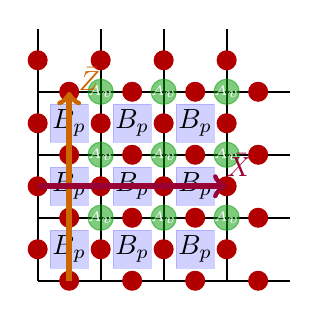
\begin{tikzpicture}[scale=0.8]
  % Surface code lattice (distance-3)
  \marginnote{visual-encoding}{%
  Red circles: data qubits on edges. Blue squares: plaquette stabilizers. Green diamonds: vertex stabilizers.%
  }

  % Data qubits (circles on edges)
  \foreach \x in {0,1,2,3} {
    \foreach \y in {0,1,2,3} {
      \draw[thick] (\x,\y) -- (\x+1,\y);
      \draw[thick] (\x,\y) -- (\x,\y+1);

      \filldraw[red!70!black] (\x+0.5,\y) circle (0.15);
      \filldraw[red!70!black] (\x,\y+0.5) circle (0.15);
    }
  }

  % Plaquette stabilizers (blue squares)
  \foreach \x in {0,1,2} {
    \foreach \y in {0,1,2} {
      \filldraw[blue!60!white,opacity=0.3] (\x+0.2,\y+0.2) rectangle (\x+0.8,\y+0.8);
      \node at (\x+0.5,\y+0.5) {$B_p$};
    }
  }

  % Vertex stabilizers (green diamonds)
  \foreach \x in {1,2,3} {
    \foreach \y in {1,2,3} {
      \filldraw[green!60!black,opacity=0.5] (\x,\y) circle (0.2);
      \node[white] at (\x,\y) {\tiny $A_v$};
    }
  }

  % Logical operators
  \draw[orange!80!black,line width=2pt,->] (0.5,0) -- (0.5,3);
  \node[orange!80!black,right] at (0.5,3.2) {$\bar{Z}$};

  \draw[purple!80!black,line width=2pt,->] (0,1.5) -- (3,1.5);
  \node[purple!80!black,above] at (3.2,1.5) {$\bar{X}$};

\end{tikzpicture}
\caption{Surface code lattice (distance-3). Data qubits (red) reside on edges. Plaquette stabilizers $B_p$ (blue) measure products of $Z$ operators around faces. Vertex stabilizers $A_v$ (green) measure products of $X$ operators at vertices. Logical operators $\bar{X}, \bar{Z}$ (orange/purple) are non-contractible loops.}
\label{fig:p6:surface_code_lattice}
\end{figure}

\begin{figure}[htbp]
\centering
\begin{tikzpicture}[scale=1.2]
  % E8 lattice projection (2D slice)
  \marginnote{projection-method}{%
  Cartan subalgebra projection onto maximal torus visualizes 240 roots as vertices of Gosset polytope $4_{21}$.%
  }

  \foreach \angle in {0,15,...,345} {
    \coordinate (P\angle) at (\angle:2);
    \filldraw[blue!60!black] (P\angle) circle (0.08);
  }

  % Root vectors (12 outer vertices)
  \foreach \angle in {0,30,...,330} {
    \coordinate (R\angle) at (\angle:3);
    \filldraw[red!70!black] (R\angle) circle (0.12);
    \draw[thick,gray!50] (0,0) -- (R\angle);
  }

  % Weyl chamber sectors
  \foreach \angle in {0,30,...,330} {
    \pgfmathsetmacro{\nextangle}{\angle+30}
    \draw[blue!40,thick,dashed] (R\angle) -- (R\nextangle);
  }

  \node at (0,-3.8) {E$_8$ Root System (2D Projection)};
  \node[red!70!black,right] at (3.2,0) {Simple roots};
  \node[blue!60!black,right] at (2.2,1) {Positive roots};

\end{tikzpicture}
\caption{E$_8$ lattice root system projected onto 2D plane. Red dots: 12 simple roots. Blue dots: 240 total roots. Dashed lines: Weyl chamber boundaries. Dimensional reduction to (2+1)D yields anyon models with fusion rules derived from root multiplicities.}
\label{fig:p6:e8_lattice}
\end{figure}

\begin{figure}[htbp]
\centering
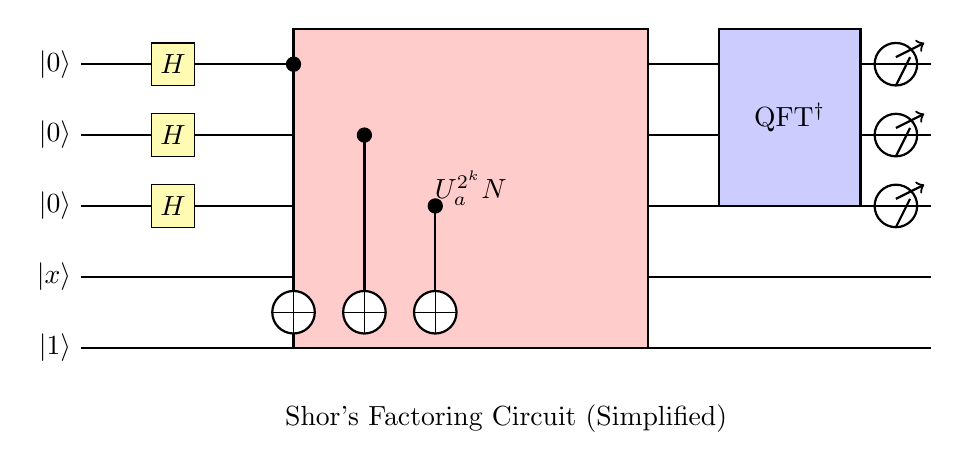
\begin{tikzpicture}[scale=0.9]
  % Quantum circuit for Shor's algorithm (simplified)
  \marginnote{circuit-notation}{%
  Wires: qubits (top = control, bottom = target). Boxes: gates. Meter symbols: measurements.%
  }

  % Qubit lines
  \foreach \y in {0,1,2,3,4} {
    \draw[thick] (0,\y) -- (12,\y);
  }

  % Labels
  \node[left] at (0,4) {$|0\rangle$};
  \node[left] at (0,3) {$|0\rangle$};
  \node[left] at (0,2) {$|0\rangle$};
  \node[left] at (0,1) {$|x\rangle$};
  \node[left] at (0,0) {$|1\rangle$};

  % Hadamard gates
  \foreach \y in {2,3,4} {
    \draw[fill=yellow!30] (1,\y-0.3) rectangle (1.6,\y+0.3);
    \node at (1.3,\y) {$H$};
  }

  % Modular exponentiation (black box)
  \draw[fill=red!20,thick] (3,0) rectangle (8,4.5);
  \node at (5.5,2.25) {$U_a^{2^k} \mod N$};

  % Controlled gates
  \foreach \k/\y in {0/4, 1/3, 2/2} {
    \draw[fill=black] (3+\k,\y) circle (0.1);
    \draw[thick] (3+\k,\y) -- (3+\k,0.5);
    \draw[fill=white,thick] (3+\k,0.5) circle (0.3);
    \draw (3+\k,0.2) -- (3+\k,0.8);
    \draw (3+\k-0.3,0.5) -- (3+\k+0.3,0.5);
  }

  % Quantum Fourier Transform
  \draw[fill=blue!20,thick] (9,2) rectangle (11,4.5);
  \node at (10,3.25) {QFT$^\dagger$};

  % Measurements
  \foreach \y in {2,3,4} {
    \draw[thick] (11.5,\y) circle (0.3);
    \draw[thick] (11.5,\y-0.3) -- (11.7,\y+0.1);
    \draw[->,thick] (11.5,\y+0.1) -- (11.9,\y+0.3);
  }

  \node at (6,-1) {Shor's Factoring Circuit (Simplified)};

\end{tikzpicture}
\caption{Quantum circuit for Shor's algorithm. Top qubits: superposition register (Hadamard gates + QFT). Middle: modular exponentiation $a^x \mod N$ via controlled unitary gates. Bottom: ancilla qubit. Measurement extracts period $r$, yielding factors of $N$.}
\label{fig:p6:shor_circuit}
\end{figure}

\begin{figure}[htbp]
\centering
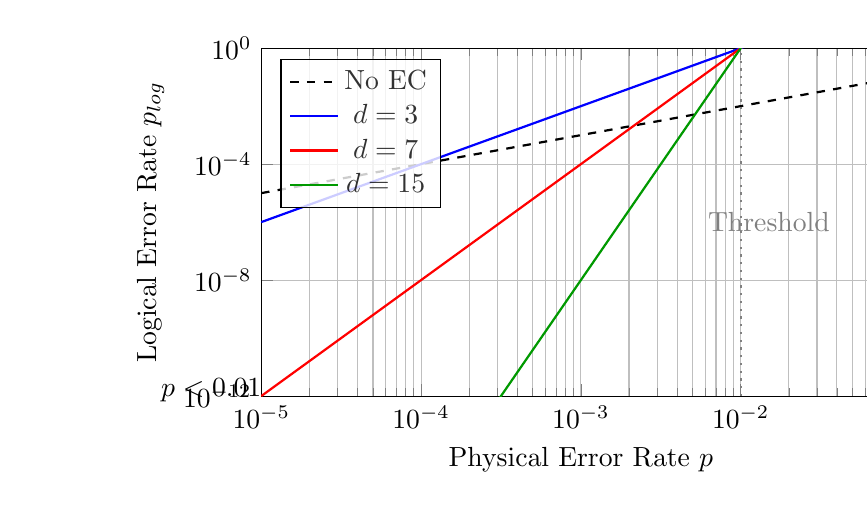
\begin{tikzpicture}
  \begin{axis}[
    width=0.8\textwidth,
    height=6cm,
    xlabel={Physical Error Rate $p$},
    ylabel={Logical Error Rate $p_{\text{log}}$},
    xmode=log,
    ymode=log,
    xmin=1e-5, xmax=1e-1,
    ymin=1e-12, ymax=1e0,
    grid=both,
    legend pos=north west,
    legend style={fill=white,fill opacity=0.8}
  ]

  \marginnote{threshold-visualization}{%
  Below threshold ($p < 0.01$), larger code distance exponentially suppresses logical errors. Above threshold, errors proliferate.%
  }

  % No error correction (identity line)
  \addplot[domain=1e-5:1e-1, samples=50, black, thick, dashed] {x};
  \addlegendentry{No EC}

  % Distance-3 code
  \addplot[domain=1e-5:1e-1, samples=50, blue, thick] {(x/0.01)^2};
  \addlegendentry{$d=3$}

  % Distance-7 code
  \addplot[domain=1e-5:1e-1, samples=50, red, thick] {(x/0.01)^4};
  \addlegendentry{$d=7$}

  % Distance-15 code
  \addplot[domain=1e-5:1e-1, samples=50, green!60!black, thick] {(x/0.01)^8};
  \addlegendentry{$d=15$}

  % Threshold line
  \addplot[domain=1e-12:1e0, samples=2, gray, thick, dotted] coordinates {(0.01,1e-12) (0.01,1e0)};
  \node[gray] at (axis cs:0.015,1e-6) {Threshold};

  \end{axis}
\end{tikzpicture}
\caption{Logical error rate vs physical error rate for surface codes. Below threshold $p_{\text{th}} \sim 1\%$, larger code distance $d$ exponentially suppresses logical errors: $p_{\text{log}} \sim (p/p_{\text{th}})^{(d+1)/2}$. Current hardware ($p \sim 10^{-3}$) approaches fault-tolerance regime.}
\label{fig:p6:error_threshold}
\end{figure}

\begin{figure}[htbp]
\centering
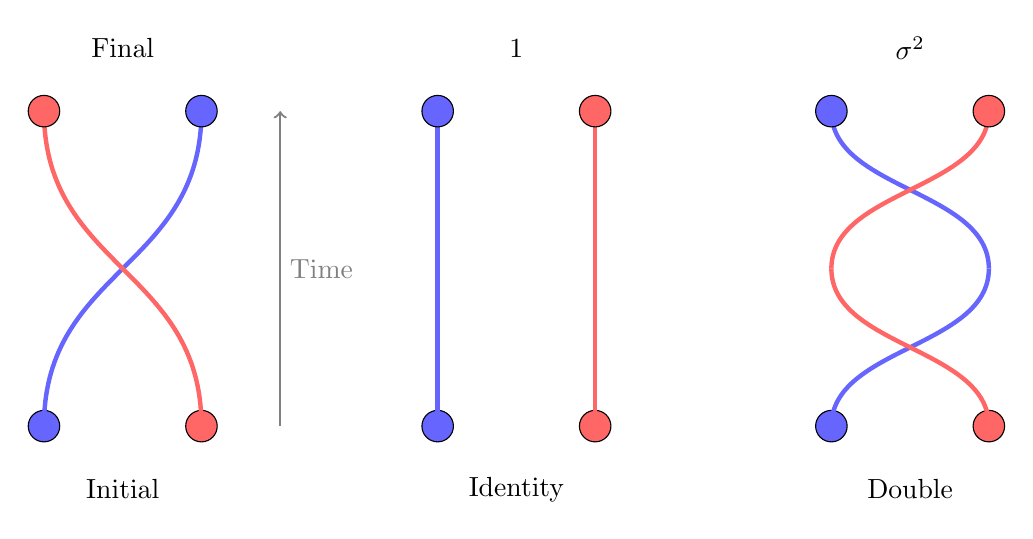
\begin{tikzpicture}
  % Topological qubit braiding
  \marginnote{braiding-topology}{%
  Worldlines (time vertical) of anyons braid in (2+1)D spacetime, tracing out knot invariants corresponding to unitary gates.%
  }

  \begin{scope}[xshift=0cm]
    % Initial state
    \draw[fill=blue!60] (0,0) circle (0.2);
    \draw[fill=red!60] (2,0) circle (0.2);
    \node at (1,-0.8) {Initial};

    % Braiding paths
    \draw[blue!60,ultra thick] (0,0) .. controls (0,2) and (2,2) .. (2,4);
    \draw[red!60,ultra thick] (2,0) .. controls (2,2) and (0,2) .. (0,4);

    % Final state
    \draw[fill=red!60] (0,4) circle (0.2);
    \draw[fill=blue!60] (2,4) circle (0.2);
    \node at (1,4.8) {Final};

    % Time axis
    \draw[->,thick,gray] (3,0) -- (3,4);
    \node[gray,right] at (3,2) {Time};
  \end{scope}

  \begin{scope}[xshift=5cm]
    % Identity (no braiding)
    \draw[fill=blue!60] (0,0) circle (0.2);
    \draw[fill=red!60] (2,0) circle (0.2);
    \node at (1,-0.8) {Identity};

    \draw[blue!60,ultra thick] (0,0) -- (0,4);
    \draw[red!60,ultra thick] (2,0) -- (2,4);

    \draw[fill=blue!60] (0,4) circle (0.2);
    \draw[fill=red!60] (2,4) circle (0.2);
    \node at (1,4.8) {$\mathbb{1}$};
  \end{scope}

  \begin{scope}[xshift=10cm]
    % Double braiding
    \draw[fill=blue!60] (0,0) circle (0.2);
    \draw[fill=red!60] (2,0) circle (0.2);
    \node at (1,-0.8) {Double};

    % First braid
    \draw[blue!60,ultra thick] (0,0) .. controls (0,1) and (2,1) .. (2,2);
    \draw[red!60,ultra thick] (2,0) .. controls (2,1) and (0,1) .. (0,2);

    % Second braid
    \draw[blue!60,ultra thick] (2,2) .. controls (2,3) and (0,3) .. (0,4);
    \draw[red!60,ultra thick] (0,2) .. controls (0,3) and (2,3) .. (2,4);

    \draw[fill=blue!60] (0,4) circle (0.2);
    \draw[fill=red!60] (2,4) circle (0.2);
    \node at (1,4.8) {$\sigma^2$};
  \end{scope}

\end{tikzpicture}
\caption{Topological qubit braiding. Left: Single exchange $\sigma$ (worldlines cross once). Middle: Identity (no exchange). Right: Double braiding $\sigma^2$. For Fibonacci anyons, $\sigma^5 = \mathbb{1}$ (finite braid group), enabling universal quantum gates via braid sequences.}
\label{fig:p6:anyon_braiding}
\end{figure}

%------------------------------------------------------------------------------
\section{Conclusion and Outlook}
%------------------------------------------------------------------------------

Quantum computing stands at an inflection point. Current hardware achieves $\sim$100-qubit systems with error rates approaching fault-tolerance thresholds, yet scaling to $10^6$ qubits required for factoring 2048-bit integers remains daunting. This chapter has outlined three advanced approaches:\marginnote{synthesis}{%
Topological codes, exceptional algebraic structures, and fractional dynamics offer complementary pathways beyond brute-force scaling.%
}

\begin{enumerate}
  \item \textbf{Topological protection:} Surface codes provide $\sim 10\times$ error suppression per distance level; E$_8$ anyons promise intrinsic fault-tolerance via non-Abelian braiding.

  \item \textbf{Algorithmic innovation:} Shor and Grover algorithms demonstrate exponential/quadratic speedups; fractional quantum walks optimize graph-based problems.

  \item \textbf{Practical implementation:} Worked example of distance-3 surface code quantifies overhead and decoding complexity.
\end{enumerate}

The path forward requires interdisciplinary advances:\marginnote{future-directions}{%
Materials science (topological superconductors), control theory (fast syndrome extraction), mathematics (optimal decoders).%
}

\begin{itemize}
  \item \textbf{Materials:} Stabilizing fractional quantum Hall states at $\nu = 5/2$ or engineering Majorana zero modes in nanowires.
  \item \textbf{Architecture:} Modular quantum processors linked by photonic interconnects, distributing error correction overhead.
  \item \textbf{Algorithms:} Variational quantum eigensolvers (VQE) for near-term quantum chemistry, quantum machine learning.
\end{itemize}

By 2035, quantum computers may achieve ``quantum advantage'' for specific tasks (optimization, simulation) if error rates drop below $10^{-4}$ and qubit counts reach $10^4$. Universal fault-tolerant systems ($10^6$ qubits, arbitrary algorithms) await 2040-2050 breakthroughs in scalable topological codes or radical new approaches.\marginnote{technology-timeline}{%
Pessimistic: 2060s. Optimistic: 2035 for domain-specific advantage. Realistic: 2040-2050 for general-purpose FTQC.%
}

The quantum computing revolution is not assured---but the physics is sound, and the potential transformative.

%==============================================================================
% END OF CHAPTER 1
%==============================================================================
